\chapter{شبیه‌سازی}
\noindent
\textbf{
	\textit{
		توصیف روند شبیه‌سازی سخت‌افزار و گام‌های اجرایی، مشاهدهٔ ورودی‌ها و خروجی‌های اصلی و میانی، مقایسه با مقادیر حاصل از اجرای کد نرم‌افزاری (مدل طلایی)، توصیف مراحل اجزای الگوریتم به همراه شکل موج‌ها، نحوهٔ عملکرد 
		\lr{Testbench}
	}
}
\pagebreak

\section{توضیح روند شبیه‌سازی سخت‌افزار و گام‌های اجرایی}
برای شبیه‌سازی سخت‌افزاری کد 
\lr{verilog}
الگوریتم 
\lr{Skein}
را در محیط شبیه‌سازی 
\lr{Modelsim}
اجرا کردیم. گام‌های اجرایی به صورت کلی برای شبیه‌سازی کد سخت‌افزاری موارد زیر بود. 
\begin{itemize}
	\item
	      مطالعه کد الگوریتم و تعیین ورودی‌ها
	\item
	      نوشتن Testbench
	\item
	      اجرای کد در محیط Modelsim با Testbench های مختلف
	\item
	      گرفتن Waveform و مقادیر خروجی (اصلی و میانی)
\end{itemize}
\section{مشاهدهٔ ورودی‌ها و خروجی‌های اصلی و میانی}
در ادامه ابتدا کد های Testbench اجرا شده بر الگوریتم و سپس Waveform
های حاصله و در انتها خروجی‌ها به صورت متنی آورده می‌شود.

\subsection{توضیح نحوهٔ عملکرد Testbench}
در ادامه ابتدا کد verilog نوشته‌شده برای  Testbench آورده  و سپس توضیحاتی دربارهٔ آن ایراد شده است. 
\pagebreak
\subsubsection{\lr{Testbench 1}}
\begin{code}
	//Master Testbench example
	
	module skein_tb;
	
	// Inputs
	reg clk;
	reg [511:0] midstate;
	reg [95:0] data;
	reg [31:0] nonce;
	
	// Outputs
	wire [511:0] hash;
	
	// Instantiate the Unit Under Test (UUT)
	skein512 uut (
	.clk(clk), 
	.midstate(midstate), 
	.data(data), 
	.nonce(nonce), 
	.hash(hash)
	);
	
	initial begin
	// Initialize Inputs
	clk = 0;
	midstate = 0;
	data = 0;
	nonce = 0;
	
	// Wait 100 ns for global reset to finish
	#1000
	data = 512'd12345609823;
	midstate = 96'd456;
	nonce = 32'd453;
	#1000;    
	data = 512'd7659432094555543122297600000000654;
	midstate = 96'd456;
	nonce = 32'd453;
	
	end
	always 
	#1 clk = ~clk;
	endmodule
\end{code}
\pagebreak
\subsubsection{\lr{Testbench 2}}
\begin{code}
module skein_tb;

  // Inputs
  reg clk;
  reg [511:0] midstate;
  reg [95:0] data;
  reg [31:0] nonce;

  // Outputs
  wire [511:0] hash;

  // Instantiate the Unit Under Test (UUT)
  skein512 uut (
    .clk(clk), 
    .midstate(midstate), 
    .data(data), 
    .nonce(nonce), 
    .hash(hash)
  );

  initial begin
    // Initialize Inputs
    clk = 0;
    midstate = 0;
    data = 0;
    nonce = 0;

    // Wait 100 ns for global reset to finish
    #1000
          data = "FF";
    #5000;    
  end
   always 
    #1 clk = ~clk;
      
endmodule
\end{code}


\subsection{شکل موج حاصل از Testbench}

\subsubsection{\lr{Waveform 1}}
\begin{figure}[H]
	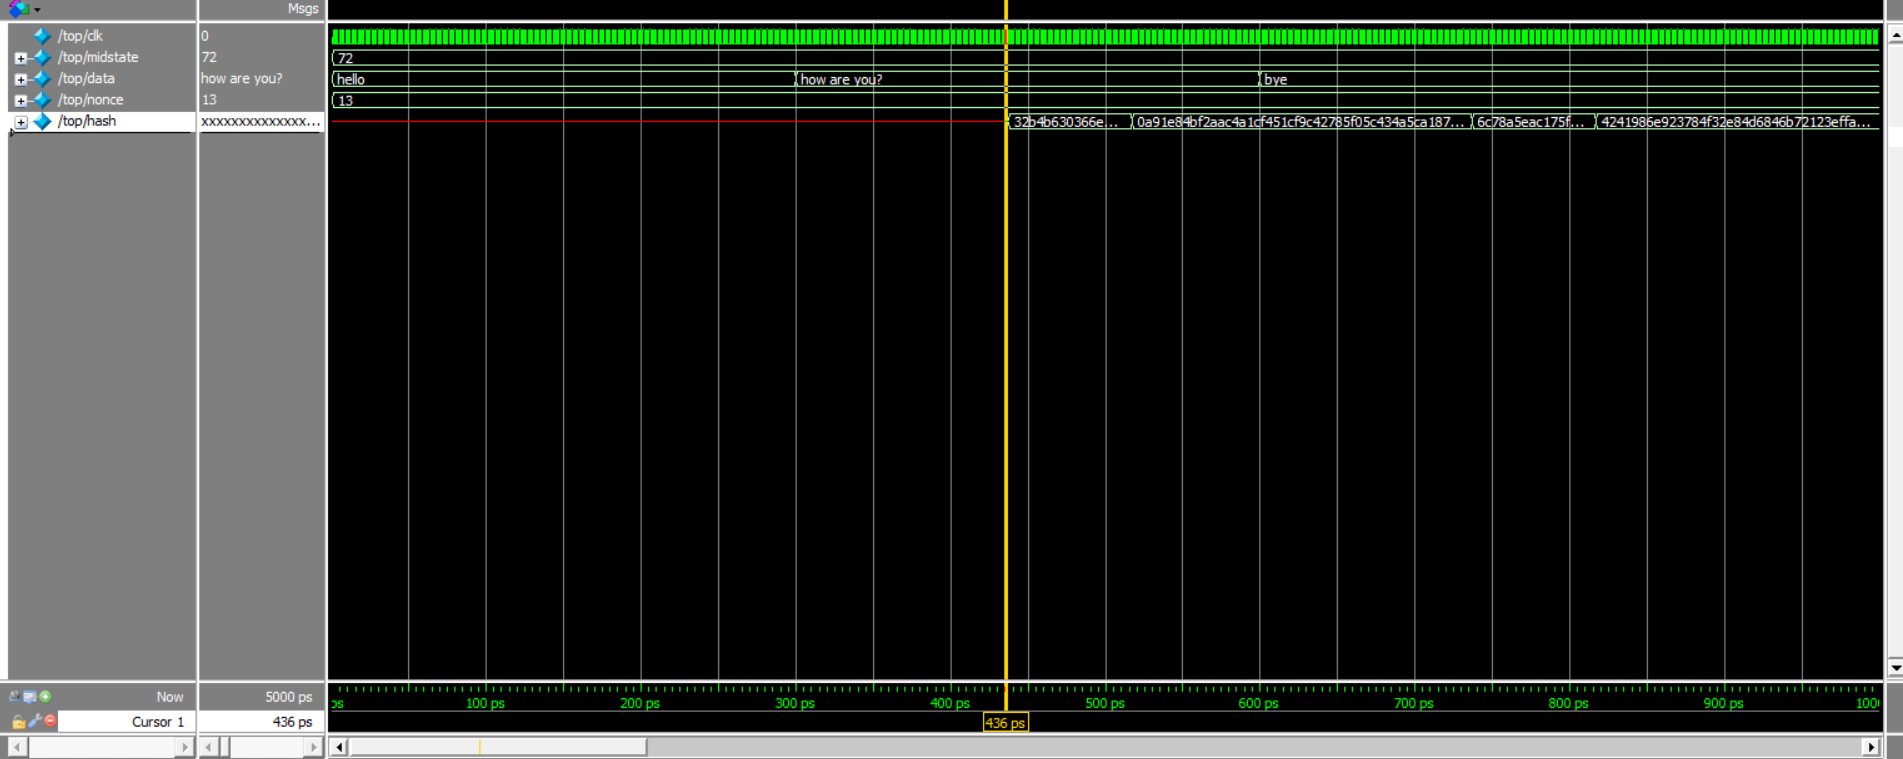
\includegraphics[width = \textwidth]{figs/simulation/1.png}
	\caption{شبیه‌سازی با \lr{Testbench 1}}
	\label{simulation_1}
\end{figure}

\subsubsection{\lr{Waveform 2}}
\begin{figure}[H]
	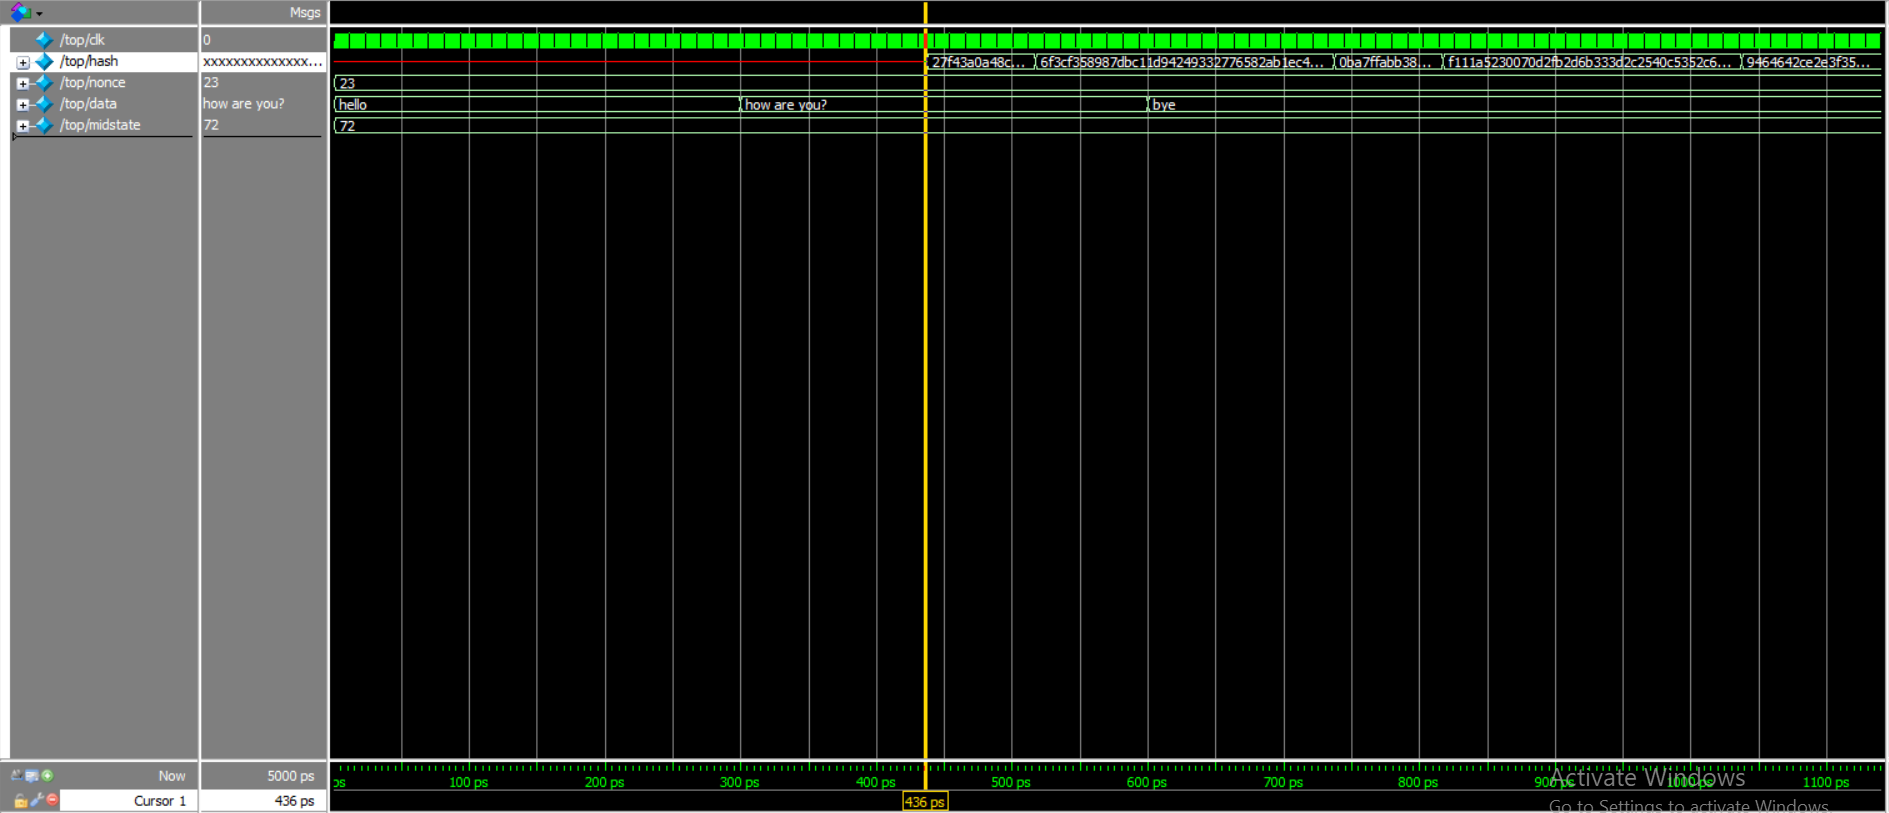
\includegraphics[width = \textwidth]{figs/simulation/2.png}
	\caption{شبیه‌سازی با \lr{Testbench 2}}
	\label{simulation_2}
\end{figure}

\subsection{جدول ورودی‌ها و خروجی‌های  Testbench}
\lr{
	\begin{table}[H]
		\resizebox{\textwidth}{!}{%
			\begin{tabular}{@{}llll@{}}
				\toprule
				Midstate & Nonce   & Data                                    & Time (clk)  \\ \midrule
				0        & 0       & 0                                       & 1000 - 0    \\
				96'd456  & 32'd453 & 512'd12345609823                        & 2000 - 1000 \\
				96'd456  & 32'd453 & 512'd7659432094555543122297600000000654 & End - 2000  \\ \bottomrule
			\end{tabular}%
		}
		\rl{
			\caption{مقادیر ورودی‌ها و زمان برای \lr{Testbench 1} }}
		\label{table_input_1}
	\end{table}}

\lr{
	\begin{table}[H]
	\centering
			\begin{tabular}{@{}llll@{}}
				\toprule
				Midstate & Nonce   & Data                                    & Time (clk)  \\ \midrule
				0        & 0       & 0                                       & 1000 - 0    \\
				0	     & 0       & FF                       				 & End - 1000 \\ \bottomrule
			\end{tabular}%
		\rl{
			\caption{مقادیر ورودی‌ها و زمان برای \lr{Testbench 2} }}
		\label{table_input_2}
	\end{table}}

\lr{
	\begin{table}[H]
		\resizebox{\textwidth}{!}{%
			\begin{tabular}{@{}ll@{}}
				\toprule
				 Hash & Time                                                                                       \\ \midrule
				\begin{tabular}[c]{@{}l@{}}ab5283d68df053ac62d053789d4b45b81a02c959d7cab97fc43451166351f117 \\ f949fe918475f762ba80567046338211461648316d4432e6c505edc3b5ee6ff5\end{tabular} & 1217 - 433        \\
				\begin{tabular}[c]{@{}l@{}}dd477bfb0f07e299560b050c7aedb947bad77571f9a7d886a06f197a55f7946b \\ 8a9cecbb948a5478380168f8bfaf8e6d7d828459564973272b18cdf99d0234f2\end{tabular} & 1436 - 1217       \\
				\begin{tabular}[c]{@{}l@{}}0c0dea4dfd9994c6eb97f500589565239347be8a5b2e4ce4832c6cc9095baa51 \\ bf2bdde45ef619f4086e71e7d86f637314357e6d20632c31612f5424644cc223\end{tabular} & 2217 - 1436       \\
				\begin{tabular}[c]{@{}l@{}}6d383e0cceb223c20c45b816a165072ad200b8091682e8e5c31295ee62ca3719 \\ afbd493a4b85859d1cbe08d98bf01e66be18f3d3536987eeef06cc7965851bf8\end{tabular} & 2437 - 2217       \\
				\begin{tabular}[c]{@{}l@{}}6b722c1b1fb150c850e02ee44e03a447401ca4ac3cde4de6eb95b2e853d0d34b \\ 53583685f4b21f9b98229734756d7b835e46c2f589e461ab7c3177fb7e572b64\end{tabular} & End - 2437        \\ \bottomrule
			\end{tabular}%
		}
		\rl{
			\caption{مقادیر درهم‌سازی و زمان  برای \lr{Testbench 1}}}
		\label{table_hash_1}
	\end{table}}
	
\lr{
	\begin{table}[H]
		\resizebox{\textwidth}{!}{%
			\begin{tabular}{@{}ll@{}}
				\toprule
				Hash & Time                                                                                       \\ \midrule
				\begin{tabular}[c]{@{}l@{}}ab5283d68df053ac62d053789d4b45b81a02c959d7cab97fc43451166351f117 \\ f949fe918475f762ba80567046338211461648316d4432e6c505edc3b5ee6ff5\end{tabular} & 1217 - 433        \\
				\begin{tabular}[c]{@{}l@{}}5e63442c883739354bfbf8008368ac0c09c61fa86b430b2864bdfe41bf48dd9b\\
8f653c22f3b712ad81f285ce4e81ca5083a9edcc07f7ddfdb0748e5b8fca57a7\end{tabular} & 1436 - 1217       \\
				\begin{tabular}[c]{@{}l@{}}05f1df792b8b2322f3385ca477b829742688da8ef5a28af41be55da9e46374da\\
580009173c55979ac88129b408773af6a92cd56f5ba4b48bc631b1f9c2e345d5\end{tabular} & End - 1436        \\
			    \bottomrule
			\end{tabular}%
		}
		\rl{
			\caption{مقادیر درهم‌سازی و زمان برای \lr{Testbench 2}}}
		\label{table_hash_2}
	\end{table}}


\pagebreak
\section{اجرا و تحلیل کد نرم‌افزاری (مدل طلایی)}
به همراه پروژه کد C الگوریتم Skein نیز به عنوان مدل طلایی ارائه شد، در ادامه مختصرا کد C مدل طلایی را تحلیل می‌کنیم.
\subsection{تحلیل کد C}
تابع $skeinhash$ با گرفتن ورودی $data$ که به صورت آرایه ای از $unsigned char$  و $output$ که به صورت آرایه‌ای از  $uint8\_t$ میباشد شروع می کند.با فراخواندن $sph\_skein512\_init$ که ورودی از جنس $sph\_skein\_big-contex$ می گیرد و سپس $sph\_skein512$ که ورودی $sph\_skein\_big-contex$ و داده و طول داده را می گیرد و در آخر $sph\_skein512\_close$ که خروجی و $sph\_skein\_big-context$ را به عنوان ورودی دارد کار خود را پایان می دهد و نتیجه را در آرایه خروجی به طول ۳۲ کپی می‌کند.\\
	در ابتدا $sph\_skein\_big-context$ بررسی می شود:
	زمینه ای برای محاسبه ی اسکین شامل مقادیر واسطه و بخشی از داده از آخرین بلوک وارد شده است.
\begin{ccode}
#ifndef DOXYGEN_IGNORE
	unsigned char buf[64];    /* first field, for alignment */
	size_t ptr; 
	sph_u64 h0, h1, h2, h3, h4, h5, h6, h7;
	sph_u64 bcount;
#endif
} sph_skein_big_context;
\end{ccode}
\begin{itemize}
\item
$buf$\\ آرایه ای به طول ۶۴ که بخش به بخش داداه را در خود ذخیره می‌کند و روی آن پردازش انجام می‌شود.
\item
$ptr$\\ سایز بخش اشغال شده بافر
\item
$h0..h7$\\$(uint64_t)$استفاده می‌شود.UBI برای محاسبه در :$h0, ..., h7$
 \item
 تعداد بلاک های داده\\$bcount$
\end{itemize}
تابع $skein\_big\_init$ مقادیر  $sph\_skein\_big-context$ که از این به بعد از آن به اختصار $ctx$ یاد میشود را مقدار دهی اولیه کرده و تمامی مقادیر آن را به جز بافر صفر می‌گذارد.\\
تابع $sph\_skein512$ بخش اصلی محاسبات را به عهده دارد.اگر سایز بافر $ctx$ خالی مانده بیشتر از طول داده باشد داده در آن کپی می‌شود.\\
سپس مقادیر $ctx$ توسط تابع $READ\_STATE\_BIG$ به روز رسانی می‌شوند و با مشخص کردن مقدار $first$ که بعدتر از آن استفاده میکند و برابر با متغیر$ first$ در $UBI$  می‌باشد با استفاده از $bcount$ زمینه که در ابتدا برابر با $0$ است ،وارد لوپ محاسبه می‌شود.\\
اگر بافر پر شده باشد، $bcount$ به علاوه یک شده و $first$  و $ptr$ صفر می‌شوند. تابع $UBI\_BIG$ با ورودی $96+first$ و $0$ فراخوانی می‌شود که همان
\lr{ The Unique Block Iteration (UBI) chaining mode}
 است که یک مقدار زنجیره ای ورودی را با یک رشته ورودی با طول اختیاری ترکیب می کند و خروجی با طول ثابت را تولید می کند.\\
.بلوک های پیام $M0$ و $M1$ و …و $M7$ هرکدام گنجایش 64 بیت داده را دارند که به ترتیب توسط  بافر$ ctx$ پر می‌شوند.\\
 مقدار $p0…p7$ مربوط به threefish که متن ساده، یک رشته از بایت های با طولی برابر با کلید، است برابر $m0..m7$ قرار می‌گیرد.\\
دو متغیر $t0$ و $t1(threefish tweak)$ با استفاده از $bcount$  که متعلق به $ctx$ است و ورودی های تابع  $UBI\_BIG$ محاسبه میشوند و تابع $TFBIG\_KINIT$با ورودی های $h0 …h7 $مربوط به $ctx$ و $t0$ و $t1$ که قبلتر محاسبه شد فراخوانی میشود که با استفاده از آن و $TFBIG\_ADDKEY$ که با هم نقش  threefish اسکین را به عهده دارند $h0..h7$ مقدار دهی میشوند.به طوری که $hn = mn \textasciicircum pn$.\\
 و این مرحله تا وقتی داده ای که در بافر نرفته باقی  مانده ادامه دارد و سپس تمامی مقادیر $ctx$ در آن نوشته میشوند.(به جز بافر)\\
 خروجی را در بافر ارائه شده میریزد و به پردازش خاتمه میدهد. زمینه یا $ctx$ به طور خودکار دوباره مقدار دهی اولیه می‌شود.ورودی این تابع به جز زمینه و آرایه‌ی خروجی،تعداد بیت های اضافه $n$ و خود بیت های اضافه $ub $میباشد که خود تابع دو ورودی آخر را مشخص می‌کند.اگر $n $صفر نباشد مقدار $x$ ای با استفاده از این دو تولید میشود که$ sph\_skein512$ آن فراخوانی میشود.در این مرحله، اگر $ptr == 0$ یعنی پیام خالی است؛ در غیر این صورت، بین 1 تا 64 بایت وجود دارد که هنوز پردازش نشده اند. در هر صورت بافر باید به یک بلوک کامل پر شده با صفر تبدیل شود(مشخصه Skein می گوید که پیام خالی پوشیده شده است تا حداقل یک بلوک برای پردازش وجود داشته باشد).
  هنگامی که این بلوک پردازش شده است، این فرآیند دوباره با بلوک پر از صفر، برای خروجی (آن بلوک encoding "0"، بیش از 8 بایت و سپس با صفر پر شده) انجام می شود.\\
  همانطور که در شکل 
  \ref{skein_normal_hash}
   میبینیم اسکین بر اساس چندین فراخوانی UBI ساخته شده است.
نتیجه  محاسبات بلوک پیکربندی UBI برای تمام پیام‌ها ثابت است و می تواند به صورت IV از پیش محاسبه شود.
\begin{figure}[H]
\centering
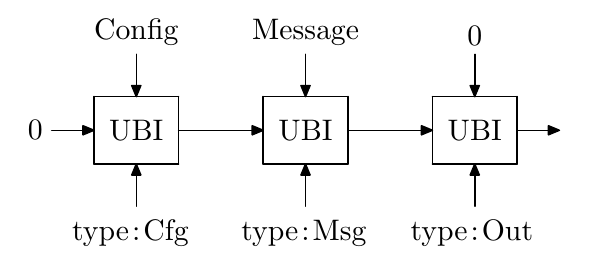
\includegraphics[scale=0.7]{figs/skein_normal_hash.png}
\caption{نحوه کار Skein}
\label{skein_normal_hash}
\end{figure}

\begin{ccode}
static const sph_u64 IV512[] = {
	SPH_C64(0x4903ADFF749C51CE), SPH_C64(0x0D95DE399746DF03),
	SPH_C64(0x8FD1934127C79BCE), SPH_C64(0x9A255629FF352CB1),
	SPH_C64(0x5DB62599DF6CA7B0), SPH_C64(0xEABE394CA9D5C3F4),
	SPH_C64(0x991112C71A75B523), SPH_C64(0xAE18A40B660FCC33)
};
\end{ccode}
\pagebreak
\subsection{مشاهدهٔ خروجی‌های کد C}
کد C که به همراه پروژه قرار داشت را اجرا کردیم، در ادامه تصویری از کد اجراشده و جدول خروجی‌های آن آمده است. 
\begin{ccode}
#include "miner.h"

#include <stdio.h>
#include <stdlib.h>
#include <stdint.h>
#include <string.h>
#include<time.h>
#include "sph_skein.h"



 void skeinhash(void *output, const void *input)
{
	uint8_t hash[64];
	sph_skein512_context ctx;
	
	sph_skein512_init(&ctx);
	sph_skein512(&ctx, input,80);
	sph_skein512_close(&ctx, (void*)hash);

	
	memcpy(output, hash,64);
}
void delay(unsigned int milliseconds){
    
    clock_t start = clock();
    
    while((clock() - start) * 1000 / CLOCKS_PER_SEC < milliseconds);
}
void print_hex(uint8_t *s, size_t len) {
    //printf("%c",len);
    for(int i = 0; i < 64; i++) {
        printf("%x", s[i]);
    }
    printf("\n");
}

int main(int argc, const char * argv[]) {
    uint8_t dst[64];
    delay(100);
    unsigned char buf[80] = "FF";
       skeinhash(dst, buf);
    for(int i = 0; i < 64; i++) {
        printf("%x", dst[i]);
        printf(" ");
    }
      printf("\n");
  
    return 0;
}
\end{ccode}
\pagebreak
\begin{figure}[H]
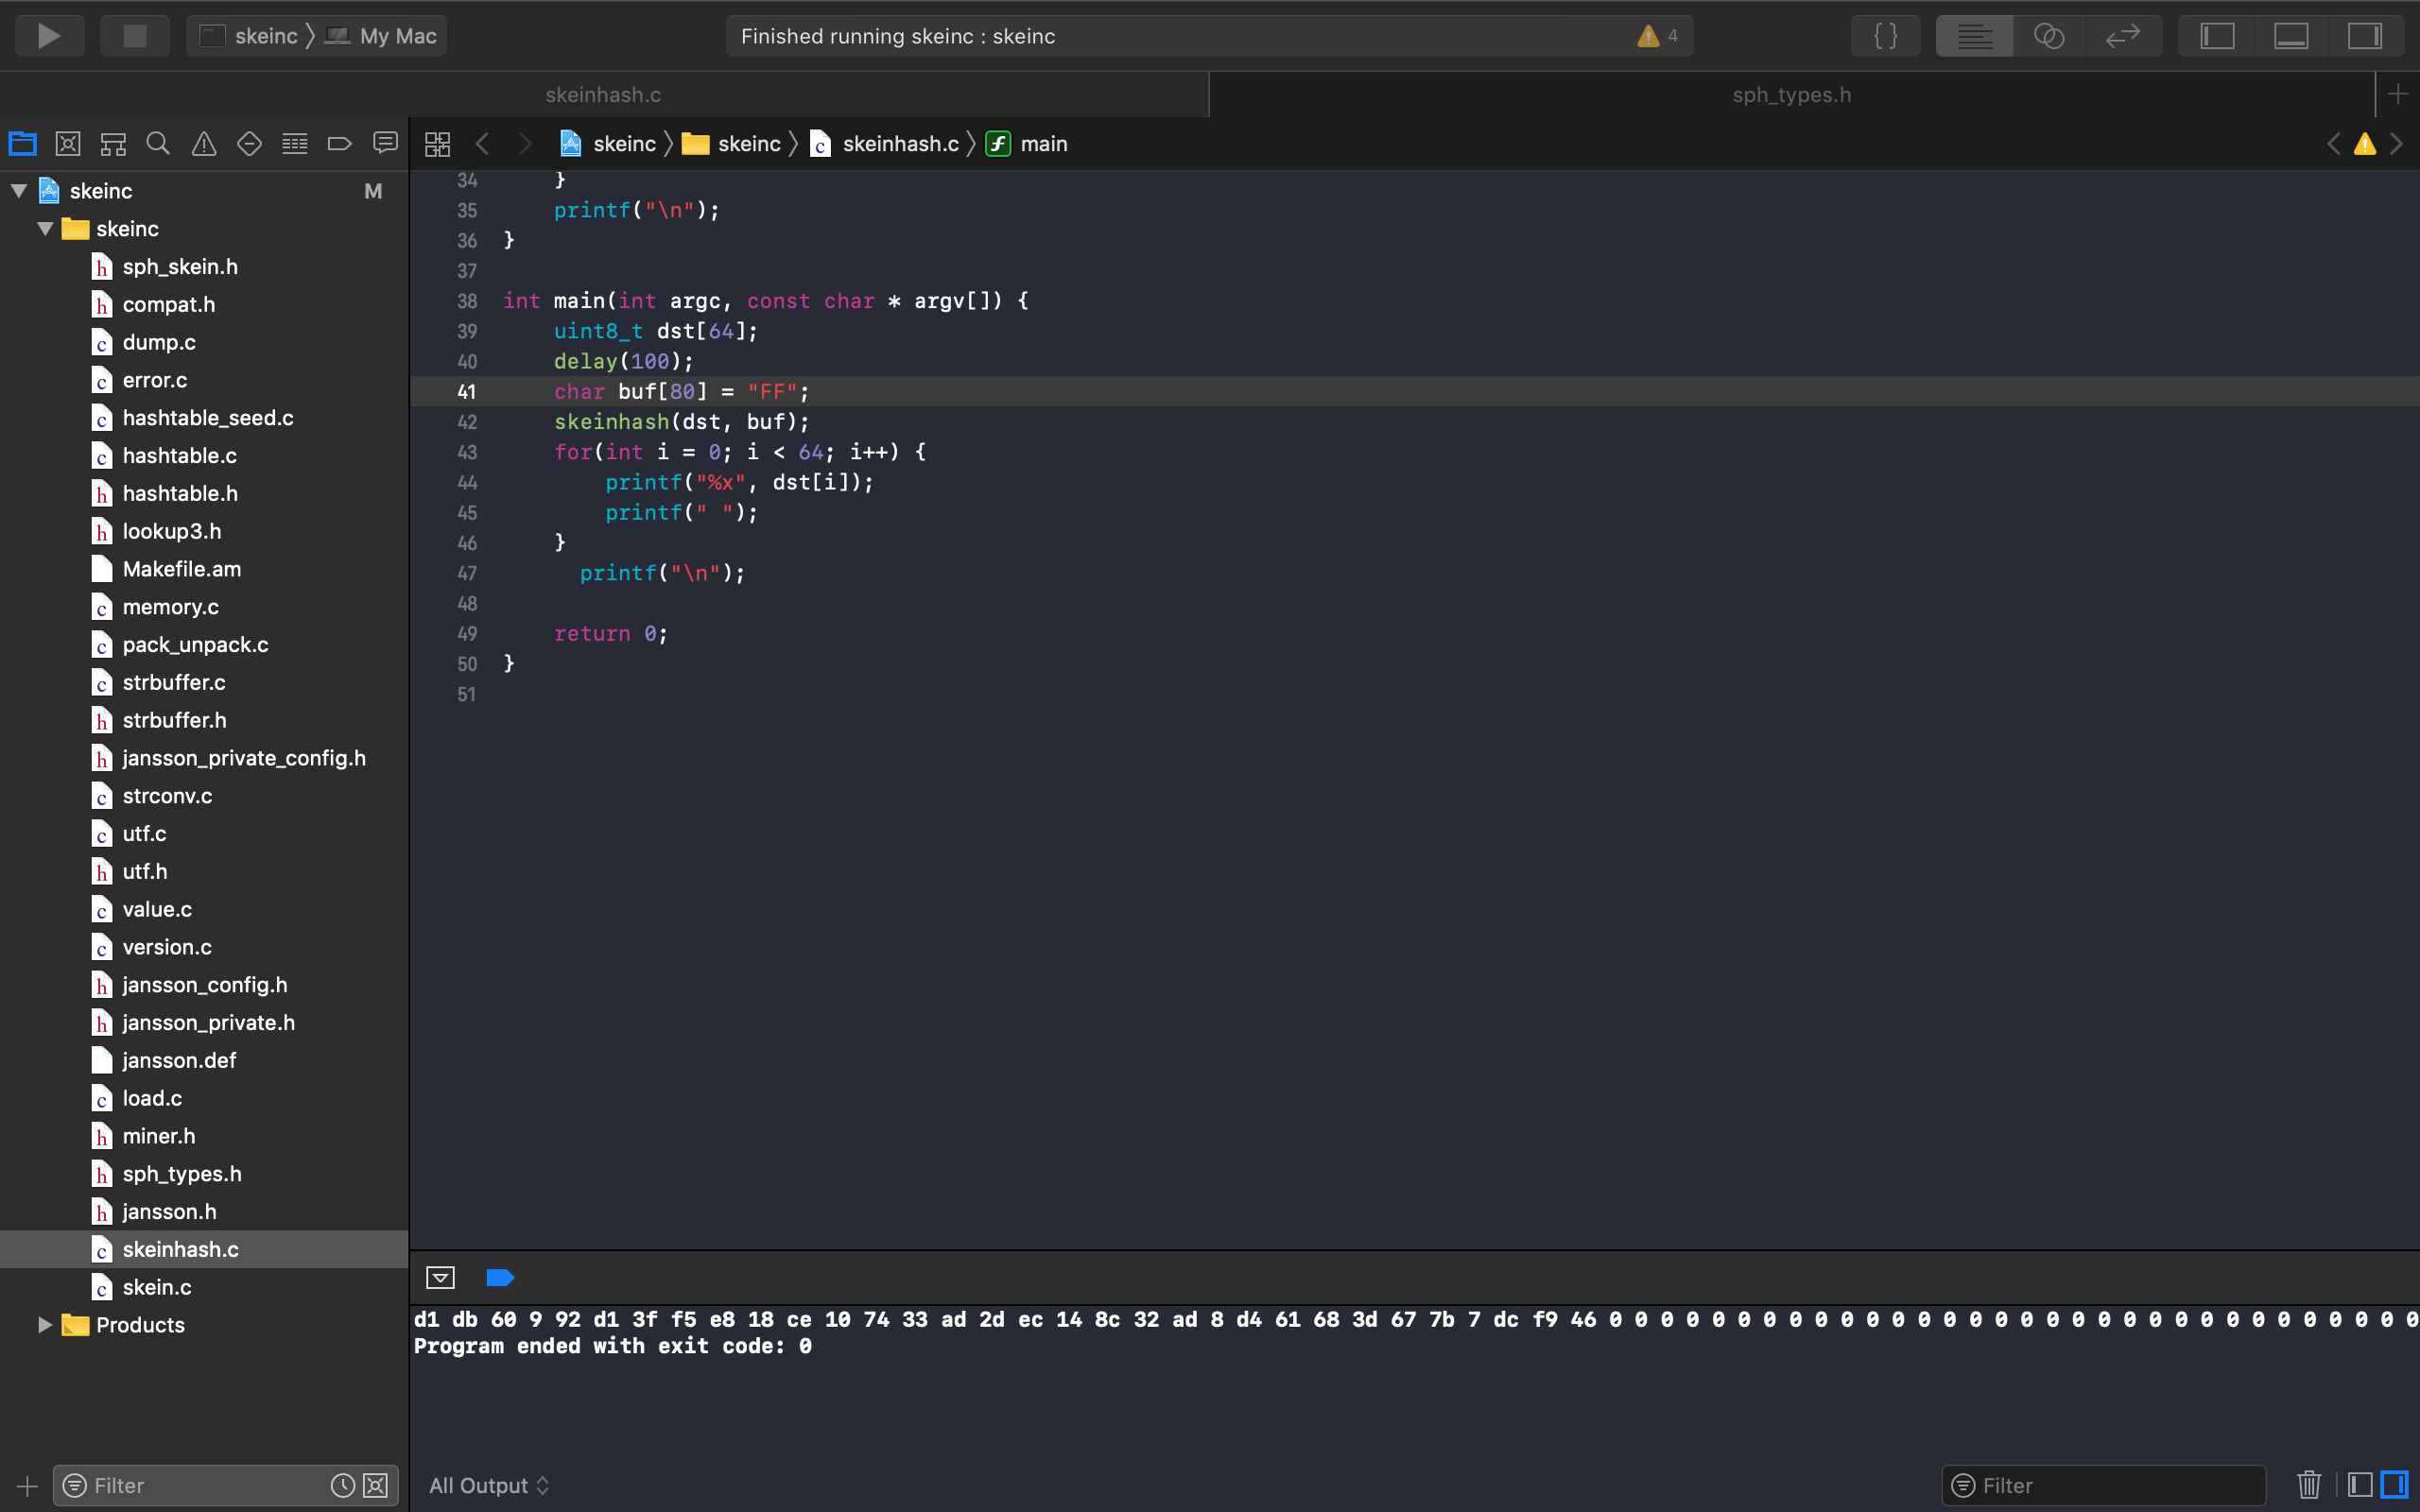
\includegraphics[width= \textwidth]{figs/simulation/output1.png}
\caption{اجرای کد C}
\label{c_output_1}
\end{figure}



\begin{figure}[H]
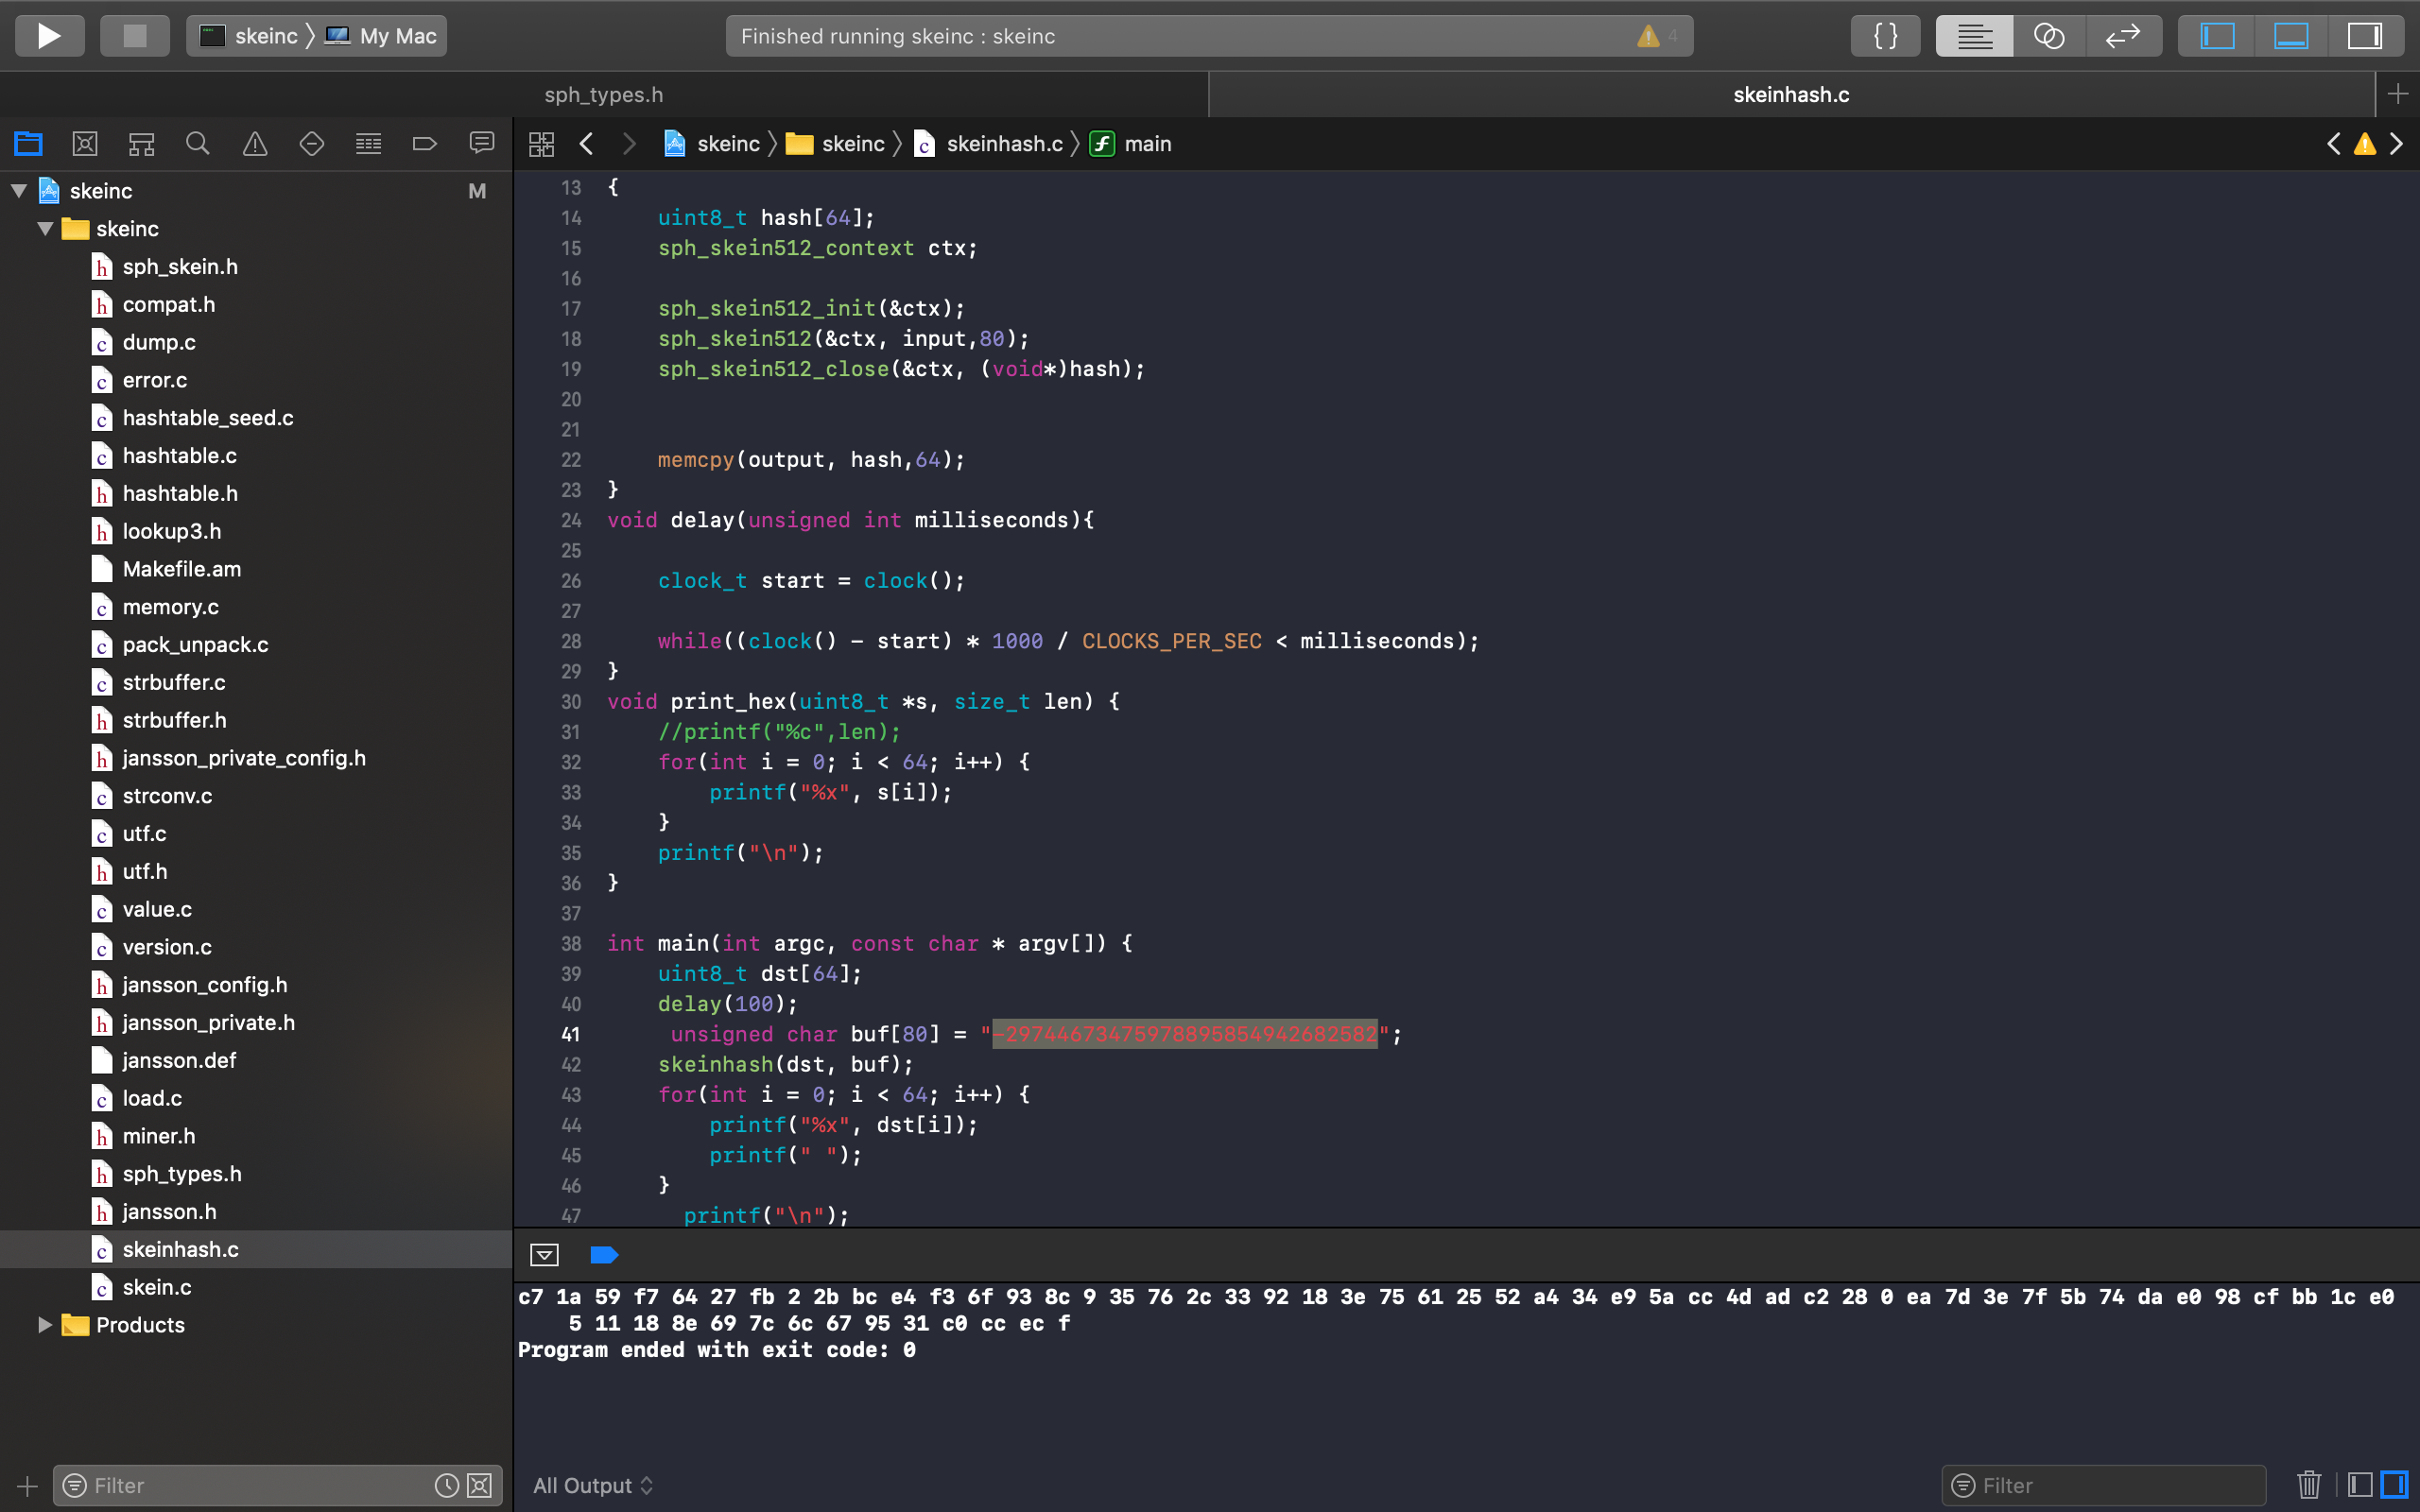
\includegraphics[width= \textwidth]{figs/simulation/output2.png}
\caption{اجرای کد C}
\label{c_output_2}
\end{figure}

\subsubsection{\lr{Output 1}}
\lr{
\begin{table}[H]
\resizebox{\textwidth}{!}{%
\begin{tabular}{@{}ll@{}}
\toprule
output & input \\ \midrule
\begin{tabular}[c]{@{}l@{}}c71a59f76427fb022bbce4f36f938c0935762c3392183e75612552a434e95acc\\
4dadc22800ea7d3e7f5b74dae098cfbb1ce00511188e697c6c679531c0ccec0f\end{tabular} & -29744673475978895854942682582 \\
\begin{tabular}[c]{@{}l@{}}d1db600992d13ff5e818ce107433ad2dec148c32ad08d461683d677b07dcf946\\
96ce76430dc7206bf3a0f37212f67b901bbdce4ee2e01b8cb214d08930df9ab7\end{tabular} & FF \\ \bottomrule
\end{tabular}
}
\rl{\caption{جدول ورودی و خروجی‌های مدل طلایی}}
\label{table_c_output_1}
\end{table}}

\subsection{مقایسه کد verilog با مدل طلایی و مرجع اصلی الگوریتم}
همان‌طور که در خروجی‌های کد C و verilog مشهود است یکی از دو کد مدل طلایی یا کد سخت‌افزاری داری اشکالاتی‌ست که منجر به تفاوت خروجی می‌شود، طبق بررسی‌های انجام‌شده کد C با کد اصلی الگوریتم تطابق دارد و نتیجتا اشکال از کد verilog است. در ادامه مشکلات یافت‌شده در کد verilog ذکر خواهد شد. 

\subsection{مقایسه خروجی کد اصلی با داکیومنت مرجع}
یکی از ورودی‌ها همانند ورودی‌ مثال در داکیومنت مرجع داده شد اما خروجی‌ها یکی نبود، خروجی داکیومنت مرجع در ادامه آمده است، تیم پروژه موفق به یافت علت تفاوت در پاسخ‌ها نشد. 

\lr{
\begin{table}[H]
\resizebox{\textwidth}{!}{%
\begin{tabular}{@{}ll@{}}
\toprule
output & input \\ \midrule
\begin{tabular}[c]{@{}l@{}}71B7BCE6FE6452227B9CED6014249E5BF9A9754C3AD618CCC4E0AAE16B316CC\\
8CA698D864307ED3E80B6EF1570812AC5272DC409B5A012DF2A579102F340617A\end{tabular} & FF \\ \bottomrule
\end{tabular}
}
\rl{\caption{جدول ورودی و خروجی‌های مستند مرجع}}
\label{table_c_output_1}
\end{table}}
\subsection{اصلاحالات موردنیاز کد verilog}
در ابتدا لازم به ذکر است که تلاش شده تا الگوریتم با الگوریتم داکیومنت اصلی که توسط طراحان الگوریتم طراحی شده مطابقت داده شود، تمامی ارجاعات داخل متن به \\
	\lr{The Skein Hash Function Family\\
		Version 1.3 — 1 Oct 2010\\
		http://www.skein-hash.info/sites/default/files/skein1.3.pdf\\
	}
	خواهد بود. 
\par
در ماژول های چهارگانه $skein\_round\_x$ در اساینمنت $pkx$ ها 
( $k$ متغیر )
عمل $MIX$ در حال انجام است. به این شکل که برای $k$ های زوج جمع ساده دو کلمه از ورودی و برای $k$ های فرد با توجه به مقدار $even$، عمل $left-rotation$ انجام میشود و سپس با یکی از $k$ های زوج $xor$ میشود تا به خروجی متصل شود.
$Left-rotaion$ به اندازه $x$ یعنی همه ی بیت های یک کلمه (64 بیتی) به اندازه $x$ بیت به سمت چپ منتقل شوند و بیت هایی که از مرز سمت چپ کلمه (بیت 64 ام) بیرون میزنند، از سمت راست با همان ترتیب وارد میشوند.\\
 در ماژول های $skein\_round\_2$ در خط 416 و $skein\_round\_4$ در خط 502 assignment های مربوط به $p3x$ و $p7x$ با توجه به جدول شماره 4 از صفحه 11 منبع ذکر شده، جابه‌جا نوشته شده اند و نیاز است تصحیح شود.\\
 عبارت صحیح برای $skein\_round\_2$ :
 \begin{code}
 	//Modification of skein_round_2
 	assign p0x = p0 + p3;
	assign p1x = (even) ? { p1[30:0], p1[63:31] } : { p1[50:0], p1[63:51] };
	assign p2x = p2 + p1;
	assign p3x = (even) ? { p3[36:0], p3[63:37] } : { p3[13:0], p3[63:14] };
	assign p4x = p4 + p7;
	assign p5x = (even) ? { p5[49:0], p5[63:50] } : { p5[53:0], p5[63:54] }
	assign p6x = p6 + p5;
	assign p7x = (even) ? { p7[21:0], p7[63:22] } : { p7[46:0], p7[63:47] };
 \end{code}
  عبارت صحیح برای $skein\_round\_4$ :
\begin{code}
	//Modification of skein_round_4
	assign p0x = p0 + p7;
	assign p1x = (even) ? { p1[19:0], p1[63:20] } : { p1[55:0], p1[63:56] };
	assign p2x = p2 + p5;
	assign p3x = (even) ? { p3[54:0], p3[63:55] } : { p3[28:0], p3[63:29] };
	assign p4x = p4 + p3;
	assign p5x = (even) ? { p5[ 9:0], p5[63:10] } : { p5[ 7:0], p5[63: 8] };
	assign p6x = p6 + p1;
	assign p7x = (even) ? { p7[ 7:0], p7[63: 8] } : { p7[41:0], p7[63:42] };
\end{code}
در ماژول های $skein\_round\_x$ (هر چهار ماژول) حین اتصال کردن $pkx$ ها به $out$ از روند خاصی که درجدول شماره 3 صفحه 11 منبع ذکر شده باید پیروی کرد.\\
با توجه به اعداد مربوط به ماژول های 8 کلمه ای، خروجی ها را باید به $pkx$ های مناسب متصل کرد که در ماژول ها رعایت نشده است.\\
محتویات $always-block$ داخل هر چهار ماژول $skein\_round\_x$ باید شکل زیر تغییر کند:
\begin{code}
	//Modificaiotion of skein_round_x ( x = 1,2,3,4)	
	out [511:448] <= p2x;
	out[447:384] <= p0x ^ p1x;
	out[383:320] <= p4x;
	out[319:256] <= p6x ^ p7x;
	out[255:192] <= p6x;
	out[191:128] <= p4x ^ p3x;
	out[127: 64] <= p0x;
	out[ 63:  0] <= p2x ^ p3x;
\end{code}
